

\begin{frame}
\frametitle{Coral Reef}
\hspace{1.57em}Coral reefs serve as a complex aquatic ecosystem physically supported by calcium carbonate secretions of the colorful stone coral. To model this ecosystem, one approach taken by Li-Wang-Zhang-Hastings is to describe the relationships between macroalgae, algal turfs, and corals \cite{Hastings}.
\end{frame}

\begin{frame}
\frametitle{Coral Reef Ecosystem}
\hspace{1.57em}
\end{frame}

\begin{frame}
\frametitle{Coral Reef Dynamics}
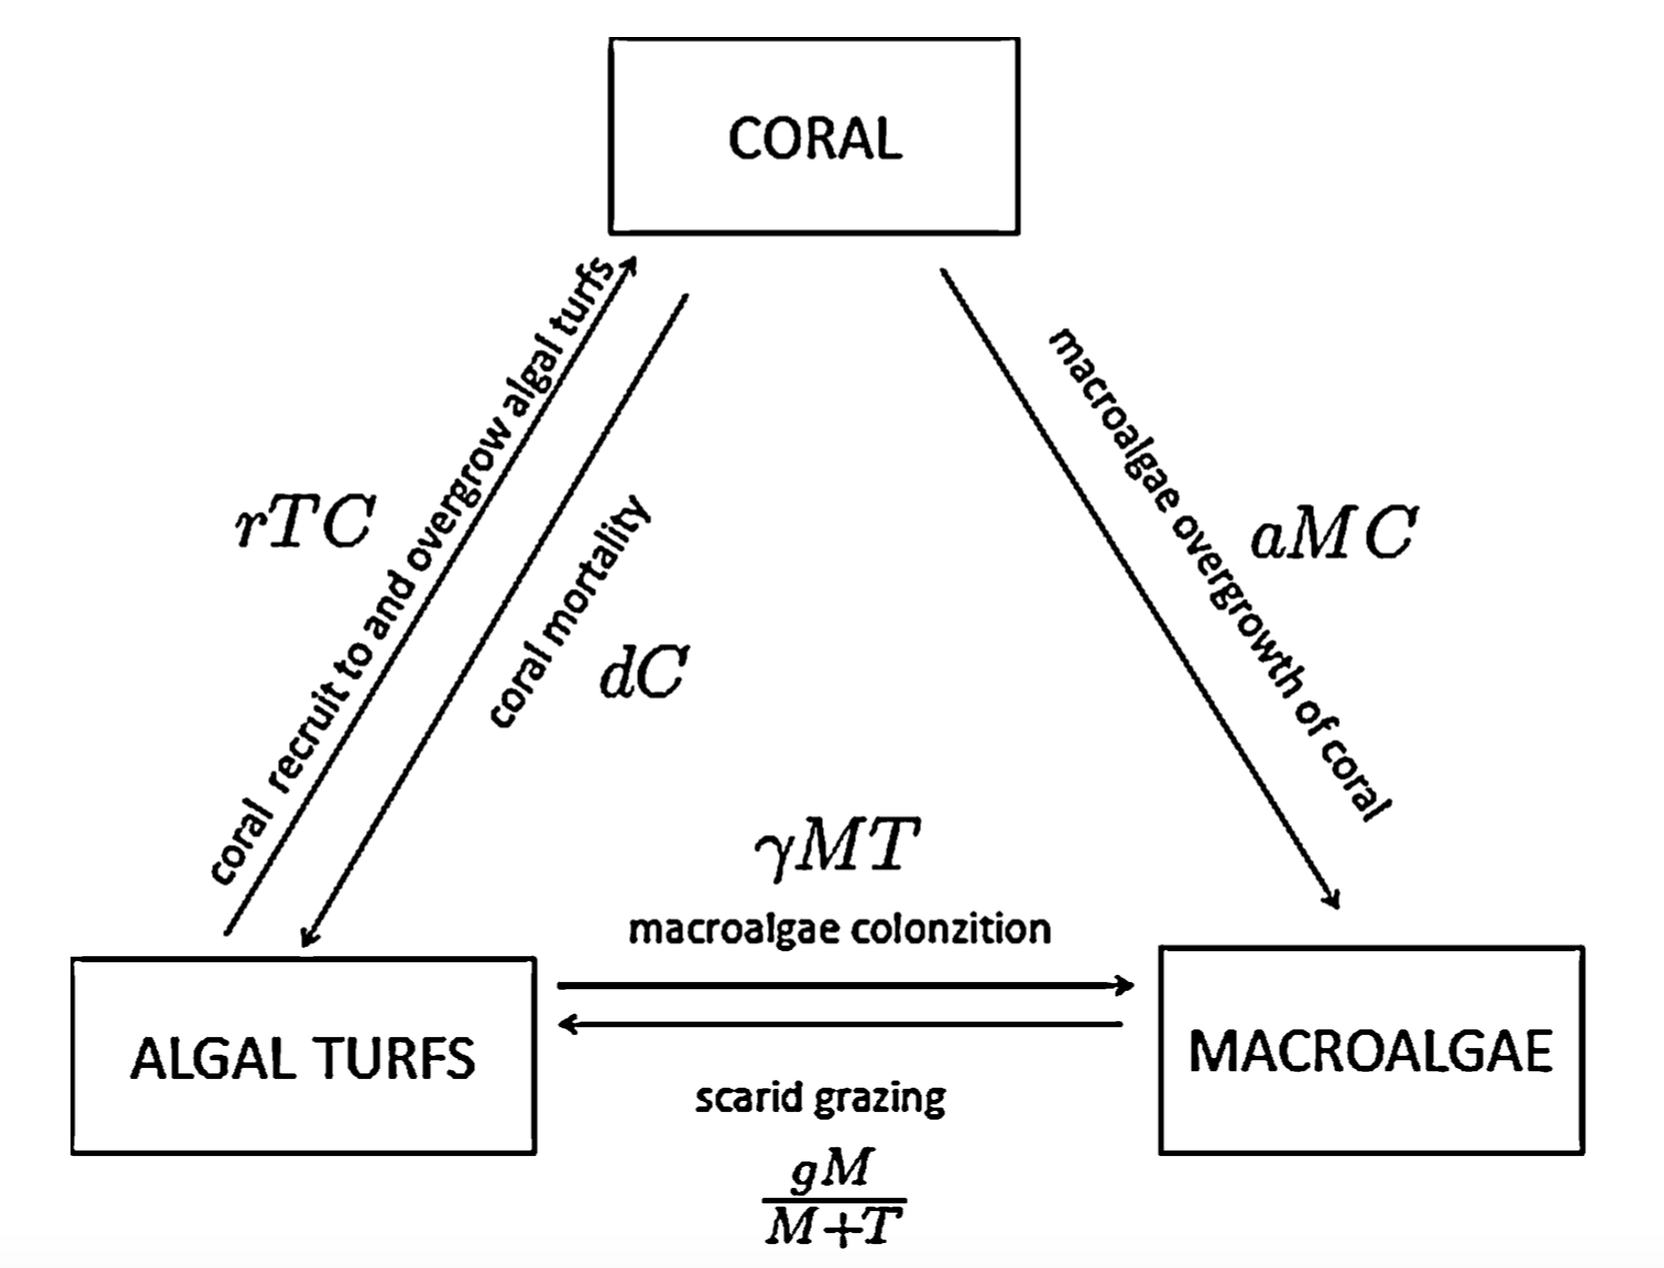
\includegraphics[scale=.175]{./coral-reef-triangle.png}
\end{frame}

\begin{frame}\frametitle{Coral Reef Dynamics}
The ordinary differential equation model:
$$\begin{cases}\begin{array}{rl}
\frac{dM}{dt}\hspace{-.8em}&=aMC - \frac{gM}{M+T} + \gamma M T\\
\frac{dC}{dt}\hspace{-.8em}&=rTC - dC - aMC\\
\frac{dT}{dt}\hspace{-.8em}&=\frac{gM}{M + T} - \gamma MT - rTC + dC
\end{array}\end{cases},$$ where \begin{itemize}\itemsep0pt
\item $r$ is the rate corals overgrow upon algal turfs\\
\item $d$ is the mortality rate of corals\\
\item $a$ is the rate that macroalgae overgrow upon corals\\
\item $\gamma$ is the rate that macroalgae spread over algal turfs\\
\item $g$ is the indiscriminate grazing rate of parrotfish.
\end{itemize}
\end{frame}

\begin{frame}\frametitle{Coral Reef Dynamics}
\hspace{1.57em}Note that our scope is limited to regions entirely covered by coral, macroalgae, and algal turf, as $\frac{dT}{dt}=-\frac{dM}{dt}-\frac{dC}{dt}$ implies $M+C+T=constant$, say $constant = 1$.  We reduce our system to, $$\begin{cases} 
\begin{array}{rl}
\frac{dM}{dt}&= aMC-\frac{gM}{1-C} + \gamma M - \gamma M^2 -\gamma M C\\ 
\frac{dC}{dt}&=rC - rC^2 - rCM - dC - aMC
\end{array} \end{cases}.$$ 
\end{frame}

\begin{frame}
\frametitle{Time Delay in the Coral Ecosystem}

\end{frame}

\begin{frame}\frametitle{Coral Reef Dynamics}
Delay Differential Equation Model:
$$\begin{cases}\begin{array}{rl}
\frac{dM}{dt}\hspace{-.8em}&=aMC - \frac{gM(t-\tau)}{1-C(t-\tau)}+\gamma M T\\
\frac{dC}{dt}\hspace{-.8em}&=rTC - dC - aMC\\
\end{array}\end{cases}.$$
\end{frame}



\begin{frame}
\frametitle{Stochastic Model}
We implemented statistical noise in this model in order to account for the stochastic features of scarid grazing habits: 
$$\begin{cases}\begin{array}{rl}
\frac{dM}{dt}\hspace{-.8em}&=aMC - \frac{gM(t-\tau)}{1-C(t-\tau)}+\gamma M T+\beta M(1-M)dW\\
\frac{dC}{dt}\hspace{-.8em}&=rTC - dC - aMC\\
\end{array}\end{cases}.$$
\end{frame}


